\documentclass[a4paper,conference]{IEEEtran}
% This is stripped down to basically the ieee bare_conf.tex header
\usepackage{amssymb,amsmath}
% use upquote if available, for straight quotes in verbatim environments
\IfFileExists{upquote.sty}{\usepackage{upquote}}{}
% use microtype if available
\IfFileExists{microtype.sty}{%
\usepackage{microtype}
\UseMicrotypeSet[protrusion]{basicmath} % disable protrusion for tt fonts
}{}
\usepackage{hyperref}
\PassOptionsToPackage{usenames,dvipsnames}{color} % color is loaded by hyperref
\hypersetup{unicode=true,
            pdftitle={Limpieza y Transformación de Datos con R},
            pdfborder={0 0 0},
            breaklinks=true}
\urlstyle{same}  % don't use monospace font for urls
% -- biblio. set natbib: true in pandoc for silly hacks around pandoc \cite{} vs \citep{}
\usepackage{cite}
\bibliographystyle{IEEEtran}
\let\citep\cite
% if you want the [2, 3] vs IEEE [2], [3]
\renewcommand{\citepunct}{,\penalty\citepunctpenalty\ }
\usepackage{color}
\usepackage{fancyvrb}
\newcommand{\VerbBar}{|}
\newcommand{\VERB}{\Verb[commandchars=\\\{\}]}
\DefineVerbatimEnvironment{Highlighting}{Verbatim}{commandchars=\\\{\}}
% Add ',fontsize=\small' for more characters per line
\usepackage{framed}
\definecolor{shadecolor}{RGB}{248,248,248}
\newenvironment{Shaded}{\begin{snugshade}}{\end{snugshade}}
\newcommand{\AlertTok}[1]{\textcolor[rgb]{0.94,0.16,0.16}{#1}}
\newcommand{\AnnotationTok}[1]{\textcolor[rgb]{0.56,0.35,0.01}{\textbf{\textit{#1}}}}
\newcommand{\AttributeTok}[1]{\textcolor[rgb]{0.13,0.29,0.53}{#1}}
\newcommand{\BaseNTok}[1]{\textcolor[rgb]{0.00,0.00,0.81}{#1}}
\newcommand{\BuiltInTok}[1]{#1}
\newcommand{\CharTok}[1]{\textcolor[rgb]{0.31,0.60,0.02}{#1}}
\newcommand{\CommentTok}[1]{\textcolor[rgb]{0.56,0.35,0.01}{\textit{#1}}}
\newcommand{\CommentVarTok}[1]{\textcolor[rgb]{0.56,0.35,0.01}{\textbf{\textit{#1}}}}
\newcommand{\ConstantTok}[1]{\textcolor[rgb]{0.56,0.35,0.01}{#1}}
\newcommand{\ControlFlowTok}[1]{\textcolor[rgb]{0.13,0.29,0.53}{\textbf{#1}}}
\newcommand{\DataTypeTok}[1]{\textcolor[rgb]{0.13,0.29,0.53}{#1}}
\newcommand{\DecValTok}[1]{\textcolor[rgb]{0.00,0.00,0.81}{#1}}
\newcommand{\DocumentationTok}[1]{\textcolor[rgb]{0.56,0.35,0.01}{\textbf{\textit{#1}}}}
\newcommand{\ErrorTok}[1]{\textcolor[rgb]{0.64,0.00,0.00}{\textbf{#1}}}
\newcommand{\ExtensionTok}[1]{#1}
\newcommand{\FloatTok}[1]{\textcolor[rgb]{0.00,0.00,0.81}{#1}}
\newcommand{\FunctionTok}[1]{\textcolor[rgb]{0.13,0.29,0.53}{\textbf{#1}}}
\newcommand{\ImportTok}[1]{#1}
\newcommand{\InformationTok}[1]{\textcolor[rgb]{0.56,0.35,0.01}{\textbf{\textit{#1}}}}
\newcommand{\KeywordTok}[1]{\textcolor[rgb]{0.13,0.29,0.53}{\textbf{#1}}}
\newcommand{\NormalTok}[1]{#1}
\newcommand{\OperatorTok}[1]{\textcolor[rgb]{0.81,0.36,0.00}{\textbf{#1}}}
\newcommand{\OtherTok}[1]{\textcolor[rgb]{0.56,0.35,0.01}{#1}}
\newcommand{\PreprocessorTok}[1]{\textcolor[rgb]{0.56,0.35,0.01}{\textit{#1}}}
\newcommand{\RegionMarkerTok}[1]{#1}
\newcommand{\SpecialCharTok}[1]{\textcolor[rgb]{0.81,0.36,0.00}{\textbf{#1}}}
\newcommand{\SpecialStringTok}[1]{\textcolor[rgb]{0.31,0.60,0.02}{#1}}
\newcommand{\StringTok}[1]{\textcolor[rgb]{0.31,0.60,0.02}{#1}}
\newcommand{\VariableTok}[1]{\textcolor[rgb]{0.00,0.00,0.00}{#1}}
\newcommand{\VerbatimStringTok}[1]{\textcolor[rgb]{0.31,0.60,0.02}{#1}}
\newcommand{\WarningTok}[1]{\textcolor[rgb]{0.56,0.35,0.01}{\textbf{\textit{#1}}}}
\usepackage{graphicx,grffile}
\makeatletter
\def\maxwidth{\ifdim\Gin@nat@width>\linewidth\linewidth\else\Gin@nat@width\fi}
\def\maxheight{\ifdim\Gin@nat@height>\textheight\textheight\else\Gin@nat@height\fi}
\makeatother
% Scale images if necessary, so that they will not overflow the page
% margins by default, and it is still possible to overwrite the defaults
% using explicit options in \includegraphics[width, height, ...]{}
\setkeys{Gin}{width=\maxwidth,height=\maxheight,keepaspectratio}

\title{Limpieza y Transformación de Datos con R}
% for over three affiliations, or if they all won't fit within the width
% of the page, use this alternative format. Cannot use \and or alignment is wrong
\author{\IEEEauthorblockN{%
  Josué Romero J.\IEEEauthorrefmark{1}%
}
\IEEEauthorblockA{\IEEEauthorrefmark{1}
      Corporación Universitaria Minuto de Dios\\
      Bogatá D.C, COA Engativa, CLL 80}
\IEEEauthorblockA{\IEEEauthorrefmark{2}
      \href{mailto:josue.romero@uniminuto.edu.co}{\nolinkurl{josue.romero@uniminuto.edu.co}}'\\
      Minería de Datos \textbar{} NRC. 70348 \textbar{} Narly Sanchez}
\IEEEauthorblockA{\IEEEauthorrefmark{3}
      08 de octubre de 2024}
}





\date{2024-10-08 23:43:10 -0500}
\setlength{\parindent}{0pt}
\setlength{\parskip}{6pt plus 2pt minus 1pt}
\let\tightlist\relax % silly pandoc thing

% --- user includes
% Put your preamble here. Example.
% subfigures
\usepackage{subfig}
% dots in filenames
\usepackage{graphicx, grffile}
% bold math
\usepackage{bm}
% colours
\usepackage[usenames,dvipsnames]{xcolor}
% suppress month in bibliography
%\AtEveryBibitem{\clearfield{month}}
%\AtEveryCitekey{\clearfield{month}}

% texdef -t latex -f {cmdname} to see if cmd is already defined

% Letters in fancy font (expectation, integers, reals, normal dist)
\newcommand{\E}[1]{\operatorname{\mathbb{E}}{\left[#1\right]}}
\newcommand{\Z}{\mathbb{Z}}
\newcommand{\R}{\mathbb{R}}
\newcommand{\N}{\mathcal{N}}

\begin{document}
\maketitle
\begin{abstract}
Demostramos el uso de una plantilla RMarkdown para el estilo IEEEtran.
Por ahora es solo estilo de conferencia, pero eventualmente ampliaremos
(quizás).
\end{abstract}

\section{Introducción}\label{sec:introducciuxf3n}

Este archivo de demostración está destinado a servir como un ``archivo
de inicio'' para artículos de conferencia IEEE producidos bajo
\LaTeX~usando IEEEtran.cls versión 1.8b y posteriores. Te deseo el mayor
de los éxitos.

\hfill mds

\hfill 08 de octubre de 2024

Usa \texttt{rmarkdown::render()} para crear este documento;
esencialmente llama a \texttt{knit()} para ir de RMD a MD, y luego
\texttt{pandoc} (con todas las configuraciones en el YAML) para ir de MD
a PDF.

Se podría intentar compilar a HTML, pero por supuesto ninguno de los
estilos IEEE se aplicará. Y si se ha incluido algún \LaTeX~crudo en el
documento (como es típico en un artículo, ya que podrías necesitar el
poder adicional de \LaTeX~para proporcionar un diseño específico), esto
no se compilará en HTML.

\section{Ejemplos}\label{sec:ejemplos}

\subsection{Knitr}\label{sec:knitr}

Puedes usar knitr como de costumbre. La opción de bloque \texttt{echo=F}
debería establecerse (a menos que desees mostrar el código R en el
artículo). Además, dado que este es un diseño de dos columnas,
probablemente se desbordará, así que necesitarás

\begin{itemize}
\tightlist
\item
  ajustar el código tú mismo (por defecto knitr no ordena el código), o
\item
  habilitar el ajuste de código y especificar el ancho:
  \texttt{opts\_knit\$set(tidy=T,\ tidy.opts=list(width.cutoff=40))}.
\item
  NB: la opción de bloque \texttt{size} (por ejemplo
  \texttt{opts\_chunk\$set(size="small")}) solo funciona en Rnw, no en
  Rmd).
\end{itemize}

El ancho es bastante pequeño. Para este documento, puedes ajustar
aproximadamente 42 caracteres antes de que se desborde (ver el ejemplo
en sección~\ref{sec:figuras}).

\subsection{Figuras}\label{sec:figuras}

Por supuesto, puedes generar gráficos usando R y se insertarán con
knitr. Sin embargo, dado que knitr va de MD a RMD, se insertarán en
formato markdown, no en formato TeX. He configurado knitr para colocar
figuras en el directorio \texttt{figure/}
(\texttt{opts\_chunk\$set(fig.path=\textquotesingle{}figure/\textquotesingle{})}),
así que ahí es donde estará el gráfico.

\begin{Shaded}
\begin{Highlighting}[]
\FunctionTok{plot}\NormalTok{(Sepal.Length }\SpecialCharTok{\textasciitilde{}}\NormalTok{ Species, iris)}
\end{Highlighting}
\end{Shaded}

\begin{figure}
\centering
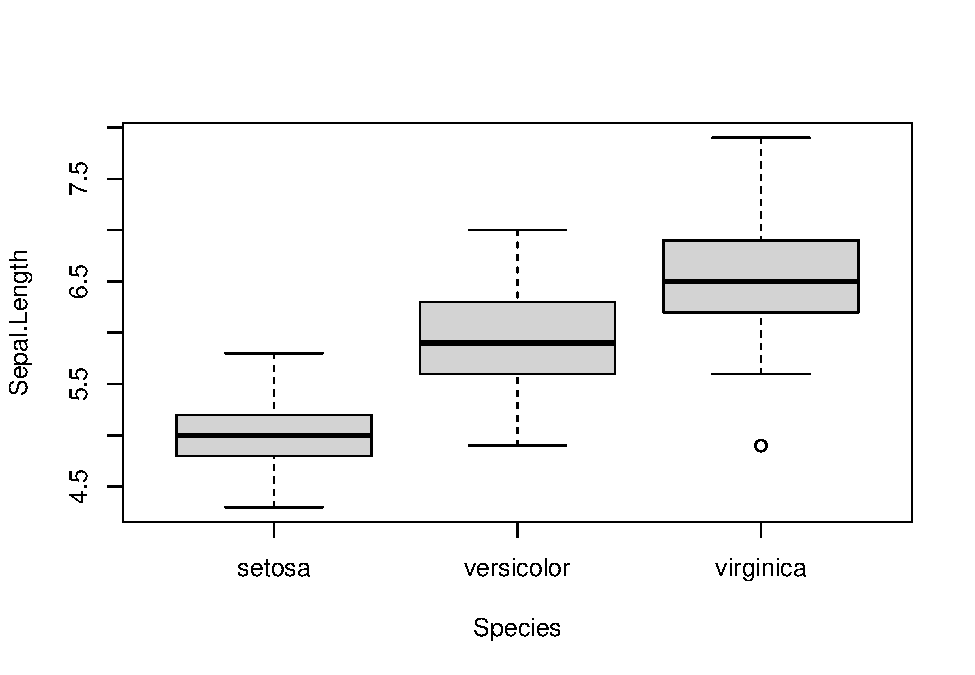
\includegraphics{figure/iris.plot-1.pdf}
\caption{Longitudes de sépalos para varias especies de
iris.\label{fig:iris}}
\end{figure}

Ver figura~\ref{fig:iris}. (No estoy seguro por qué esto es ``Fig. 1''
en la leyenda\ldots{} ¿es un asunto de knitr/rmarkdown/pandoc, o un
asunto de IEEEtran?)

En la práctica, probablemente querrás escribir tu código de figura en
\LaTeX~crudo para tener un mayor control. En el bloque de configuración
de este Rmd hay una función \texttt{latex.figure} que es un ejemplo de
salida de \LaTeX~crudo para una figura. Ajusta como desees. (Seguramente
hay una biblioteca como \texttt{xtable} para esto).

\begin{Shaded}
\begin{Highlighting}[]
\FunctionTok{latex.figure}\NormalTok{(}
  \StringTok{\textquotesingle{}figure/iris.plot{-}1.pdf\textquotesingle{}}\NormalTok{,}
  \AttributeTok{caption=}\StringTok{\textquotesingle{}Otro gráfico de longitudes de sépalos}
\StringTok{           para las diversas especies de iris.\textquotesingle{}}\NormalTok{,}
  \AttributeTok{label=}\StringTok{\textquotesingle{}fig:iris2\textquotesingle{}}\NormalTok{)}
\end{Highlighting}
\end{Shaded}

\begin{figure}[!t]%
\centering%
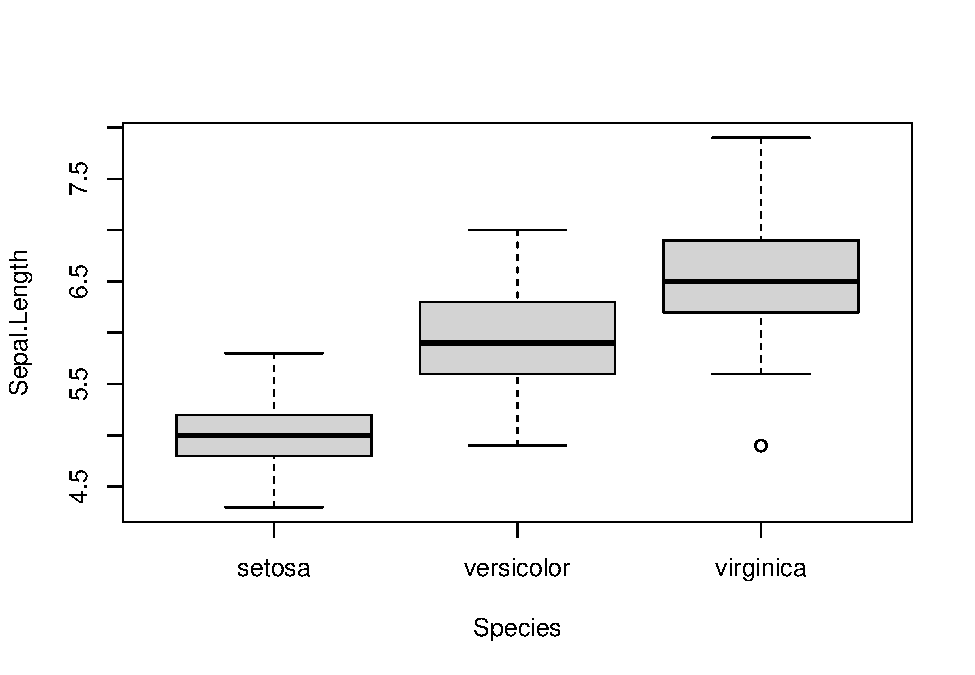
\includegraphics[width=\columnwidth]{figure/iris.plot-1.pdf}%
\caption{Otro gráfico de longitudes de sépalos
           para las diversas especies de iris.}%
\label{fig:iris2}%
\end{figure}

El comando \texttt{latex.figure} también tiene soporte básico para
subfiguras: simplemente proporciona múltiples rutas de las imágenes. Si
hay tantas leyendas como figuras, se utiliza una para cada una.\\
Si hay una leyenda más que la cantidad de figuras, la primera se usa
como la leyenda ``principal'' y el resto como leyendas de subfiguras. Si
solo hay una leyenda, se utiliza para la figura y no se añaden
subleyendas.\\
Consulta figura~\ref{fig:polinomios} para ver el resultado.

\begin{Shaded}
\begin{Highlighting}[]
\CommentTok{\# generar y guardar algunas imágenes}
\NormalTok{n }\OtherTok{=} \DecValTok{1}\SpecialCharTok{:}\DecValTok{5}
\NormalTok{figs }\OtherTok{=} \FunctionTok{sprintf}\NormalTok{(}\StringTok{\textquotesingle{}figure/x\%i.png\textquotesingle{}}\NormalTok{, n)}
\ControlFlowTok{for}\NormalTok{ (nn }\ControlFlowTok{in}\NormalTok{ n) \{}
  \FunctionTok{png}\NormalTok{(}\AttributeTok{filename=}\NormalTok{figs[nn], }\AttributeTok{width=}\DecValTok{480}\NormalTok{, }\AttributeTok{height=}\DecValTok{300}\NormalTok{)}
  \FunctionTok{plot}\NormalTok{(}\DecValTok{1}\SpecialCharTok{:}\DecValTok{10}\NormalTok{, (}\DecValTok{1}\SpecialCharTok{:}\DecValTok{10}\NormalTok{)}\SpecialCharTok{\^{}}\NormalTok{nn)}
  \FunctionTok{dev.off}\NormalTok{()}
\NormalTok{\}}

\CommentTok{\# mostrar como figura flotante con 3 subfiguras}
\FunctionTok{latex.figure}\NormalTok{(}
\NormalTok{  figs,}
  \AttributeTok{caption=}\FunctionTok{c}\NormalTok{(}\StringTok{"Polinomios"}\NormalTok{,}
            \FunctionTok{sprintf}\NormalTok{(}\StringTok{"$x\^{}\%i$"}\NormalTok{, n)),}
  \AttributeTok{label=}\StringTok{\textquotesingle{}fig:polynomials\textquotesingle{}}\NormalTok{,}
  \AttributeTok{linebreaks.after=}\DecValTok{3}\NormalTok{,}
  \AttributeTok{width=}\StringTok{\textquotesingle{}.6}\SpecialCharTok{\textbackslash{}\textbackslash{}}\StringTok{columnwidth\textquotesingle{}}\NormalTok{,}
  \AttributeTok{floating=}\NormalTok{T)}
\end{Highlighting}
\end{Shaded}

\begin{figure*}[!t]%
\centering%
\subfloat[$x^1$]{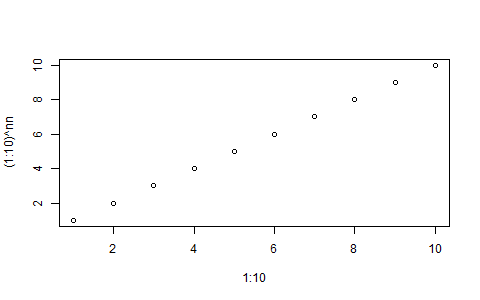
\includegraphics[width=.6\columnwidth]{figure/x1.png}}%
\subfloat[$x^2$]{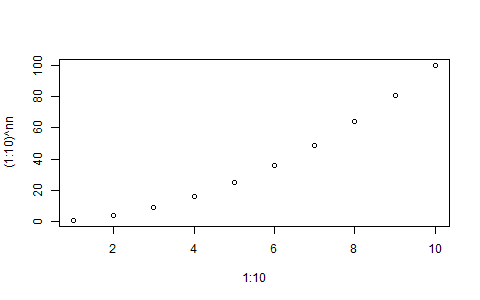
\includegraphics[width=.6\columnwidth]{figure/x2.png}}%
\subfloat[$x^3$]{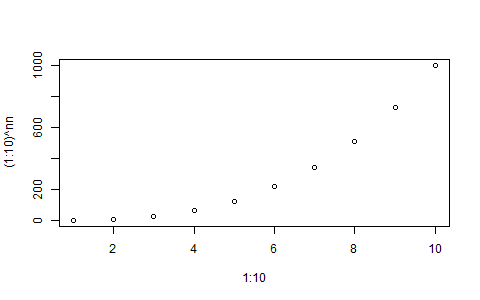
\includegraphics[width=.6\columnwidth]{figure/x3.png}}\\%
\subfloat[$x^4$]{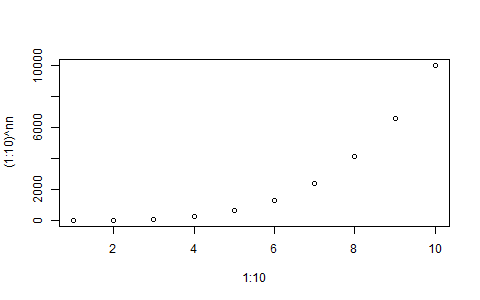
\includegraphics[width=.6\columnwidth]{figure/x4.png}}%
\subfloat[$x^5$]{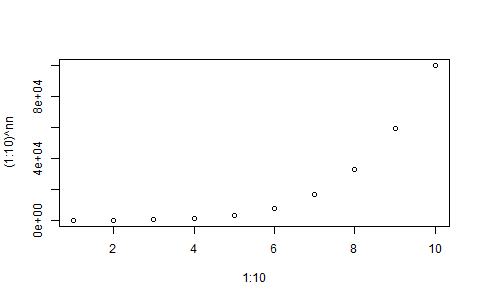
\includegraphics[width=.6\columnwidth]{figure/x5.png}}%
\caption{Polinomios}%
\label{fig:polynomials}%
\end{figure*}

Nota que frecuentemente los artículos de IEEE con subfiguras no usan
leyendas para las subfiguras, sino que en su lugar las
referencian/describen como (a), (b), etc., dentro de la leyenda
principal.

También nota que típicamente IEEE coloca los elementos flotantes solo en
la parte superior, incluso cuando esto resulta en que un gran porcentaje
de una columna esté ocupado por figuras flotantes.

\subsection{Tables}\label{sec:tables}

No debes usar la sintaxis de pandoc, ya que utiliza el paquete
\texttt{longtable} (esto está codificado) y \texttt{longtable} no
funciona bien con entradas de dos columnas. Usa algo como Hmisc o xtable
para generar salida en \LaTeX~y proporcionar mayor control (por ejemplo,
tabla~\ref{tbl:iris.xtable}).

\begin{Shaded}
\begin{Highlighting}[]
\FunctionTok{print}\NormalTok{(}\FunctionTok{xtable}\NormalTok{(}
\NormalTok{  iris[}\FunctionTok{sample}\NormalTok{(}\FunctionTok{nrow}\NormalTok{(iris), }\DecValTok{6}\NormalTok{), ],}
  \AttributeTok{caption=}\StringTok{\textquotesingle{}Ejemplo del conjunto de datos iris\textquotesingle{}}\NormalTok{,}
  \AttributeTok{label=}\StringTok{\textquotesingle{}tbl:iris.xtable\textquotesingle{}}\NormalTok{,}
  \AttributeTok{align=}\FunctionTok{c}\NormalTok{(}\FunctionTok{rep}\NormalTok{(}\StringTok{\textquotesingle{}r\textquotesingle{}}\NormalTok{, }\DecValTok{5}\NormalTok{), }\StringTok{\textquotesingle{}l\textquotesingle{}}\NormalTok{)))}
\end{Highlighting}
\end{Shaded}

\begin{table}[!t]
\centering
\caption{Ejemplo del conjunto de datos iris} 
\label{tbl:iris.xtable}
\begin{tabular}{rrrrl}
  \hline
Sepal.Length & Sepal.Width & Petal.Length & Petal.Width & Species \\ 
  \hline
7.70 & 2.60 & 6.90 & 2.30 & virginica \\ 
  5.90 & 3.00 & 5.10 & 1.80 & virginica \\ 
  5.50 & 3.50 & 1.30 & 0.20 & setosa \\ 
  5.00 & 3.50 & 1.60 & 0.60 & setosa \\ 
  6.40 & 2.80 & 5.60 & 2.20 & virginica \\ 
  5.10 & 3.70 & 1.50 & 0.40 & setosa \\ 
   \hline
\end{tabular}
\end{table}

Podrías desear que la tabla abarque varias columnas. Usa \texttt{table*}
en lugar de \texttt{table} (tabla~\ref{tbl:xtable.floating}).\\
Nota que el argumento \texttt{floating.environment} pertenece a
\texttt{print.xtable}, no a \texttt{xtable}.

\begin{Shaded}
\begin{Highlighting}[]
\FunctionTok{print}\NormalTok{(}\FunctionTok{xtable}\NormalTok{(}
    \FunctionTok{head}\NormalTok{(mtcars),}
    \AttributeTok{caption=}\StringTok{\textquotesingle{}Ejemplo del conjunto de datos}
\StringTok{             de pruebas de automóviles de motor trend\textquotesingle{}}\NormalTok{,}
    \AttributeTok{label=}\StringTok{\textquotesingle{}tbl:xtable.floating\textquotesingle{}}\NormalTok{),}
  \AttributeTok{floating.environment=}\StringTok{\textquotesingle{}table*\textquotesingle{}}\NormalTok{)}
\end{Highlighting}
\end{Shaded}

\begin{table*}[!t]
\centering
\caption{Ejemplo del conjunto de datos
             de pruebas de automóviles de motor trend} 
\label{tbl:xtable.floating}
\begin{tabular}{rrrrrrrrrrr}
  \hline
mpg & cyl & disp & hp & drat & wt & qsec & vs & am & gear & carb \\ 
  \hline
21.00 & 6.00 & 160.00 & 110.00 & 3.90 & 2.62 & 16.46 & 0.00 & 1.00 & 4.00 & 4.00 \\ 
  21.00 & 6.00 & 160.00 & 110.00 & 3.90 & 2.88 & 17.02 & 0.00 & 1.00 & 4.00 & 4.00 \\ 
  22.80 & 4.00 & 108.00 & 93.00 & 3.85 & 2.32 & 18.61 & 1.00 & 1.00 & 4.00 & 1.00 \\ 
  21.40 & 6.00 & 258.00 & 110.00 & 3.08 & 3.21 & 19.44 & 1.00 & 0.00 & 3.00 & 1.00 \\ 
  18.70 & 8.00 & 360.00 & 175.00 & 3.15 & 3.44 & 17.02 & 0.00 & 0.00 & 3.00 & 2.00 \\ 
  18.10 & 6.00 & 225.00 & 105.00 & 2.76 & 3.46 & 20.22 & 1.00 & 0.00 & 3.00 & 1.00 \\ 
   \hline
\end{tabular}
\end{table*}

Note que, para las tablas en el estilo IEEE, dado que los títulos de las
tablas funcionan como encabezados, las leyendas suelen escribirse con
mayúscula inicial en todas las palabras, excepto aquellas como: a, an,
and, as, at, but, by, for, in, nor, of, on, or, the, to y up, que
generalmente no se capitalizan, a menos que sean la primera o última
palabra de la leyenda. El texto de las tablas usará por defecto
\texttt{\textbackslash{}footnotesize}, ya que el IEEE normalmente emplea
esta fuente más pequeña para las tablas.

Note que IEEE típicamente coloca los flotantes solo en la parte
superior, incluso cuando esto resulta en que un gran porcentaje de una
columna esté ocupada por flotantes.

\subsection{Citando}\label{sec:citando}

Ejemplos de citar un autor \citep{Besag1974} y dos autores
\citep{Besag1974, Besag1986}.

\subsection{Ecuaciones}\label{sec:ecuaciones}

Son como cabría esperar. Puede utilizar la sintaxis de pandoc-crossref
para generar etiquetas. Es decir,

\begin{verbatim}
$$
e = m c^2
$$ {#eq:einstein}
\end{verbatim}

Que es igual a

\begin{equation}\phantomsection\label{eq:einstein}{
e = m c^2.
}\end{equation}

Se puede usar \texttt{@eq:einstein} para referirse a la ecuación, por
ejemplo, ~\ref{eq:einstein}. El único inconveniente es que la ecuación
debe estar en su propio párrafo si desea numerarla, lo que significa que
en el archivo tex y pdf resultante, la ecuación estará en su propia
línea. (Si no desea numerar la ecuación, no tiene que estar en su propio
párrafo y se renderizará en el párrafo como cabría esperar).

Aún no he encontrado una buena solución para esto. Es un requisito de
\texttt{pandoc-crossref}. Debe editar el archivo TeX y eliminar las
líneas en blanco adicionales (donde sea apropiado) antes de compilar.
Agrego un comentario \texttt{\%\ FIXME\ ALIGNMENT} a estas ecuaciones
para hacerlas más fáciles de encontrar.

\section{Conclusión}\label{sec:conclusiuxf3n}

Espero que se le haya dado un breve recorrido por las capacidades de
esta configuración y que ahora proceda a escribir artículos al estilo
IEEEtran utilizando RMarkdown con (relativa) facilidad.

\section*{Agradecimientos}\label{sec:agradecimientos}
\addcontentsline{toc}{section}{Agradecimientos}

Esta plantilla no sería posible sin los
\href{https://www.ctan.org/tex-archive/macros/latex/contrib/IEEEtran/?lang=en}{archivos
IEEEtran de Michael Shell}, \href{http://pandoc.org/}{pandoc},
\href{https://github.com/lierdakil/pandoc-crossref}{pandoc-crossref},
\href{http://yihui.name/knitr/}{knitr},
\href{http://rmarkdown.rstudio.com/}{rmarkdown}, y una exhaustiva
búsqueda en \href{http://stackoverflow.com/}{StackOverflow}. Merece
reconocimiento también \href{https://www.rstudio.com/}{Rstudio}. No es
necesario para esto, pero ciertamente facilita todo el proceso. Y a
cualquiera que haya olvidado mencionar.

\bibliography{IEEEabrv,./library}

\end{document}
